\section*{Overview of Supplementary Material}

This supplementary document provides comprehensive technical details, in-depth theoretical analyses, and extensive visual results to fully support the claims made in the main manuscript. The contents are systematically organized as follows:

\begin{itemize}
    \item Appendix 7: Dataset and Evaluation Protocols.
    \item Appendix 8: Extended Empirical Analyses.
    \item Appendix 9: Implementation Details.
    \item Appendix 10: User Study and Additional Qualitative Results.
\end{itemize}

\section{Dataset and Evaluation Protocols}
\subsection{Dataset Details}
% 我们使用内部构造的特效图像对进行LoRA，训练，一共收集了50个特效，每个特效的训练数据在20对左右。完整的特效信息太长不宜在pdf中直接展示，因此我们放在了附加材料压缩包的Effect.xlsx文件中。
% \begin{table}[htbp]
\centering
\caption{Examples of Teacher Prompts and the corresponding Refined Student Prompts.}
\label{tab:prompt_comparison}
\footnotesize % 减小字号以适应长文本
\renewcommand{\arraystretch}{1.3} % 稍微增加行高，提升阅读舒适度
\begin{tabularx}{\textwidth}{@{} l X X @{}}
\toprule
\textbf{LoRA Name} & \textbf{Teacher Prompt} & \textbf{Student Prompt (with Trigword)} \\
\midrule

1117\_3dshatanpangchongwu & 
Change the style to 3D realistic, change the background to a beach, change the pose to standing, and add swim trunks. & 
\textless 1117\_\allowbreak 3dshatanpangchongwu\_\allowbreak Xy5995\textgreater Transform the pet into a 3D realistic style, place it against a beach background, adjust its pose to standing, dress it in brightly colored swim trunks, maintain the fur texture, and keep the overall style cute and expressive. \\

\addlinespace % 增加行间距区分不同样本

1117\_chongwushouzhi & 
Based on the pet in the original image, retain its fur color, patterns, demeanor, expression, and body proportions, shrink it to finger size, and have it lying on a human finger. & 
\textless 1117\_\allowbreak chongwushouzhi\_\allowbreak RN8pcKDi\textgreater Based on the pet in the original image, retain its fur color, patterns, demeanor, expression, and body proportions, reduce it to finger size, place it lying on a human finger, maintain the same perspective, softly blur the background, and enhance realism and fine texture. \\

\bottomrule
\end{tabularx}
\end{table}
We utilized internally constructed special-effect image pairs for LoRA training. In total, we collected 180 distinct effects, with approximately 20 training pairs for each. 
% As the comprehensive details of these effects are too lengthy to be presented directly in this PDF, we have included them in the \textbf{Effect.xlsx} file within the supplementary materials archive.
\subsection{Prompt Design for Evaluation}
% 我们使用MLLM来评估我们的VSA和BCR指标，对于所有测试样本，我们都调用Qwen-VL-Max-Latest的API进行评估。对于BCR指标我们使用图X所示的prompt进行评估。对于VSA指标，我们先利用图X的prompt评估是否为bad case，然后再利用图X所示指标评估一致性分数。

We employ a Multimodal Large Language Model (MLLM) to evaluate our VSA and BCR metrics. Specifically, we utilize the \texttt{Qwen-VL-Max-Latest} API for the evaluation of all test samples. To assess the BCR metric, we apply the prompt detailed in Figure~\ref{fig:bcr_prompt}. For the VSA metric, we initially utilize the prompt presented in Figure~\ref{fig:bcr_prompt} to determine whether the generated result constitutes a bad case, and subsequently employ the prompt illustrated in Figure~\ref{fig:vsa_quantitative_prompt} to evaluate the consistency score.

\input{figures/BCR}
\input{figures/VSA}

\begin{figure*}[htb]
    \centering
    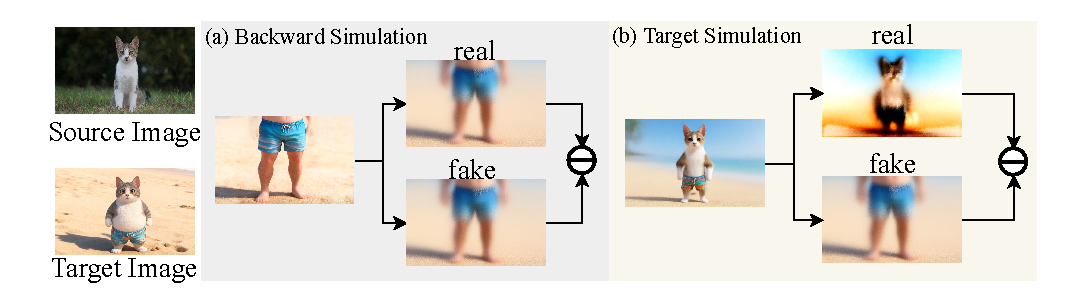
\includegraphics[width=\linewidth]{figures/grad_van.pdf}
    \caption{Comparison between (a) Backward Simulation and (b) our proposed Target Simulation. In the heterogeneous distillation setting, Backward Simulation can yield nearly identical 'real' and 'fake' predictions due to severe domain deviation, leading to the vanishing gradient problem. Conversely, Target Simulation provides distinct representations, ensuring informative gradients for the student model.}
    \label{fig:grad_van}
    \vspace{-0.5cm}
\end{figure*}

\section{Extended Empirical Analyses}
\subsection{Analysis of the Vanishing Gradient Problem}
% 梯度消失主要出现在原始DMD直接应用在异构蒸馏的设置中。在异构蒸馏设置下，学生模型和教师模型有着不完全一致的分布，学生模型要在这个过程中学习原来没有的新能力（比如特效能力）。而对于某些极端情况，学生模型通过Backward Simulation采样的结果和教师模型相差过大，会导致教师模型的输出和fake的输出几乎完全一致，导致dmd更新梯度近似为0，我们把这种现象叫做异构蒸馏的梯度消失问题。而本文提出的Target Simulation可以解决这个问题，如图X所示。
The vanishing gradient problem primarily emerges when the original DMD is directly applied in a heterogeneous distillation setting. In such a setup, the student and teacher models exhibit misaligned distributions, as the student is tasked with acquiring novel capabilities (e.g., special-effect generation) during the training process. In certain extreme cases, the samples generated by the student model via Backward Simulation deviate too drastically from the teacher model's domain. This severe discrepancy causes the teacher model's predictions to be nearly identical to the fake outputs, driving the DMD update gradient close to zero. We refer to this phenomenon as the \textit{vanishing gradient problem in heterogeneous distillation}. The Target Simulation approach proposed in this paper effectively resolves this issue, as illustrated in Figure~\ref{fig:grad_van}.





\subsection{Ablation Study on Timestep-Constrained Target Simulation}
% 引入Target Simulation后，我们进一步引入时间步约束。这一步的目的是为了放大real和fake之间的差异，从而更有效的指导学生模型更新。如图x所示，当不加时间步约束时，Target Simulation虽然不会出现梯度完全消失的问题，但是相比于引入了时间步约束的设置，明显降低了梯度更新的强度。

\begin{figure*}[htb]
    \centering
    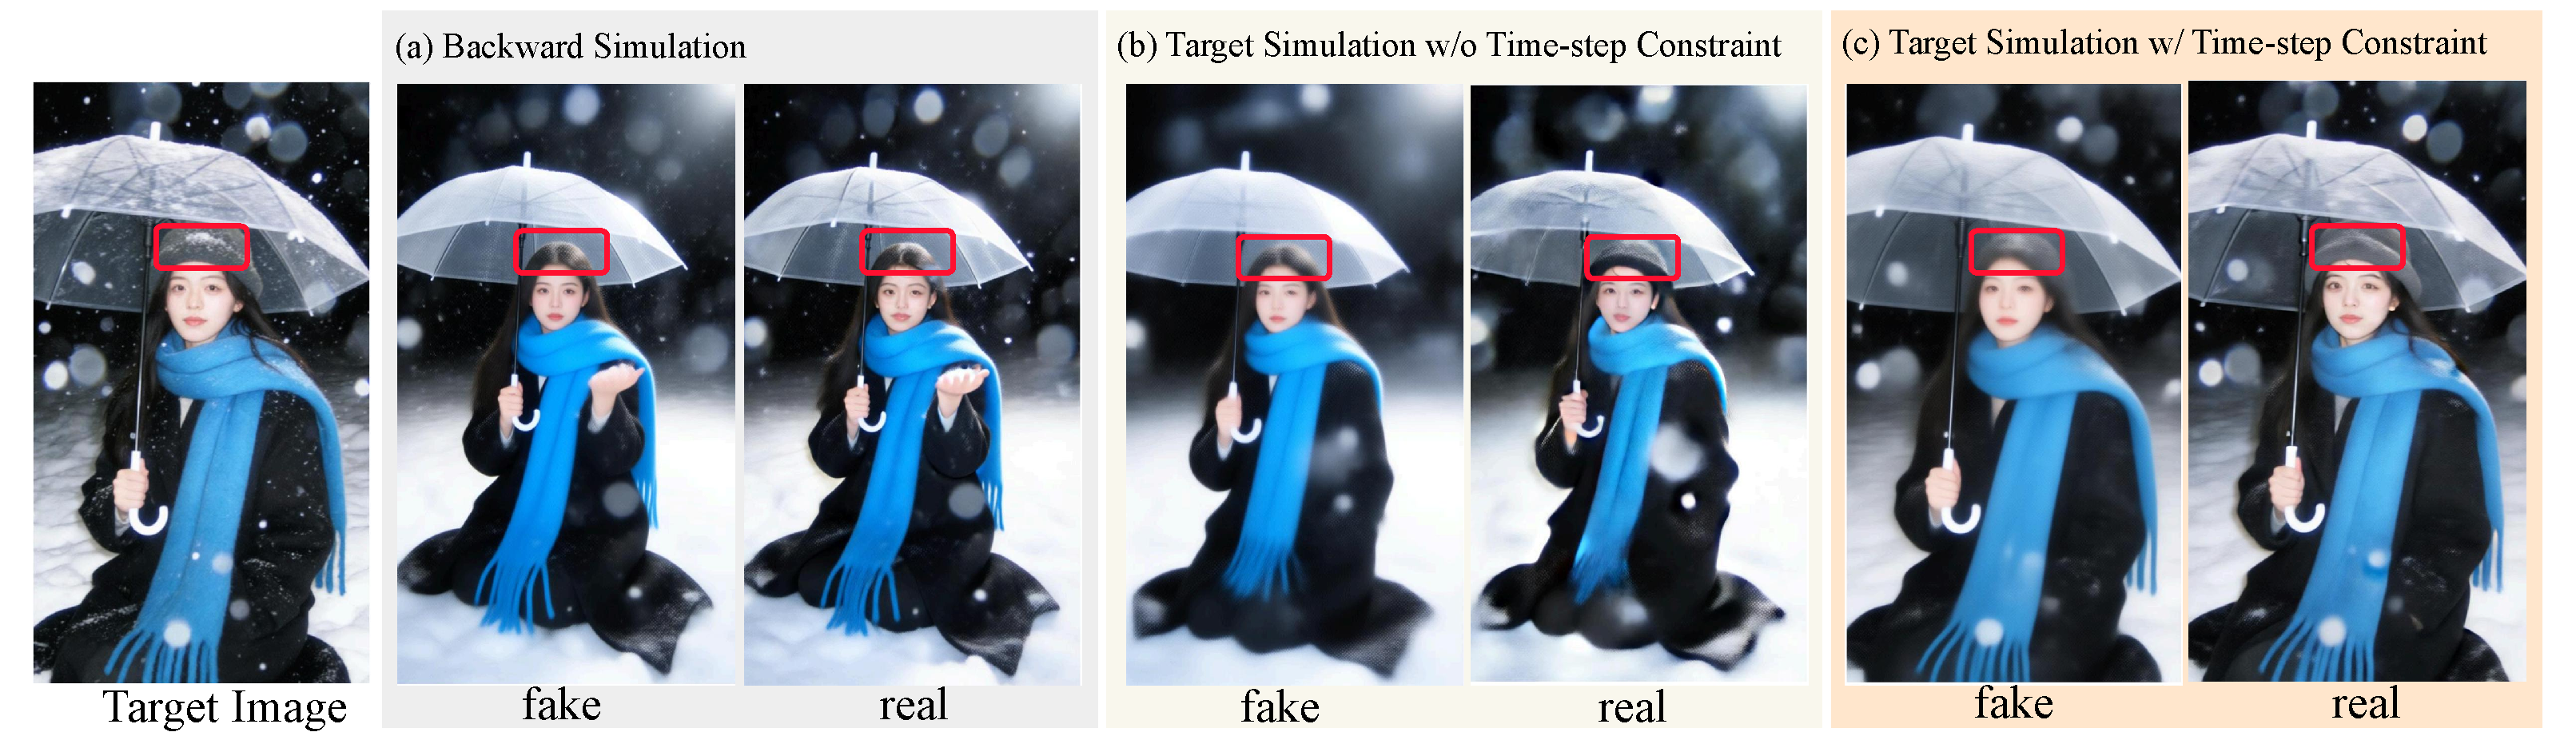
\includegraphics[width=\linewidth]{figures/zip_ablation_timestep.pdf}
    \caption{\textbf{Comparison of simulation strategies.} (a) Backward simulation leads to vanishing gradients. (b) Target simulation enables differentiation. (c) Time-step constraints further amplify the discrepancy, providing robust gradient signals for effective training.}
    \label{fig:ablation_timestep}
    \vspace{-0.5cm}
\end{figure*}

Upon the introduction of Target Simulation, we further incorporate a time-step constraint. This refinement aims to amplify the discrepancy between the ``real'' and ``fake'' predictions, thereby facilitating more effective gradient updates for the student model. As illustrated in Figure~\ref{fig:ablation_timestep}, while Target Simulation without the time-step constraint avoids the absolute vanishing gradient problem, it significantly reduces the magnitude of gradient updates compared to the setting where the constraint is imposed.



% \subsection{Training Loss Trajectories}

\section{Implementation Details}
% \subsection{Examples of Automated Asymmetric Conditioning (AAC)}
% 我们利用Qwen-VL-Max-Latest的API来为学生模型生成新的提示词。这样做既可以避免人工设计学生模型的提示词，也可以利用现成的教师模型，同时避免了多合一特效之间的提示词冲突。我们通过从训练数据中随机采样2对数据，并把教师提示词输入给MLLM来生成学生提示词，提示词模板如图X所示。我们在表X提供了几个示例用于展示。
% 单个特效训练的提示词通常为人工设计以确保更好的学到训练数据的的转换模式。通过解耦学生模型和教师模型的提示词，我们可以最大化教师的特效能力，同时开放了学生模型提示词设计的自由度。
We leverage the \texttt{Qwen-VL-Max-Latest} API to generate student prompts, which not only automates the prompt engineering process but also allows us to fully utilize existing teacher models while mitigating potential prompt conflicts in all-in-one special-effect scenarios. Specifically, we provide the MLLM with two randomly sampled training pairs and the corresponding teacher prompt to generate the refined student prompt. The prompt template is illustrated in Figure~\ref{fig:aac_prompt}, and several illustrative examples are provided in Table~\ref{tab:prompt_comparison}.
\input{figures/AAC}

\begin{table}[htbp]
\centering
\caption{Examples of Teacher Prompts and the corresponding Refined Student Prompts.}
\label{tab:prompt_comparison}
\footnotesize % 减小字号以适应长文本
\renewcommand{\arraystretch}{1.3} % 稍微增加行高，提升阅读舒适度
\begin{tabularx}{\textwidth}{@{} l X X @{}}
\toprule
\textbf{LoRA Name} & \textbf{Teacher Prompt} & \textbf{Student Prompt (with Trigword)} \\
\midrule

1117\_3dshatanpangchongwu & 
Change the style to 3D realistic, change the background to a beach, change the pose to standing, and add swim trunks. & 
\textless 1117\_\allowbreak 3dshatanpangchongwu\_\allowbreak Xy5995\textgreater Transform the pet into a 3D realistic style, place it against a beach background, adjust its pose to standing, dress it in brightly colored swim trunks, maintain the fur texture, and keep the overall style cute and expressive. \\

\addlinespace % 增加行间距区分不同样本

1117\_chongwushouzhi & 
Based on the pet in the original image, retain its fur color, patterns, demeanor, expression, and body proportions, shrink it to finger size, and have it lying on a human finger. & 
\textless 1117\_\allowbreak chongwushouzhi\_\allowbreak RN8pcKDi\textgreater Based on the pet in the original image, retain its fur color, patterns, demeanor, expression, and body proportions, reduce it to finger size, place it lying on a human finger, maintain the same perspective, softly blur the background, and enhance realism and fine texture. \\

\bottomrule
\end{tabularx}
\end{table}

% \section{User Study}

\begin{figure}[htbp]
    \centering
    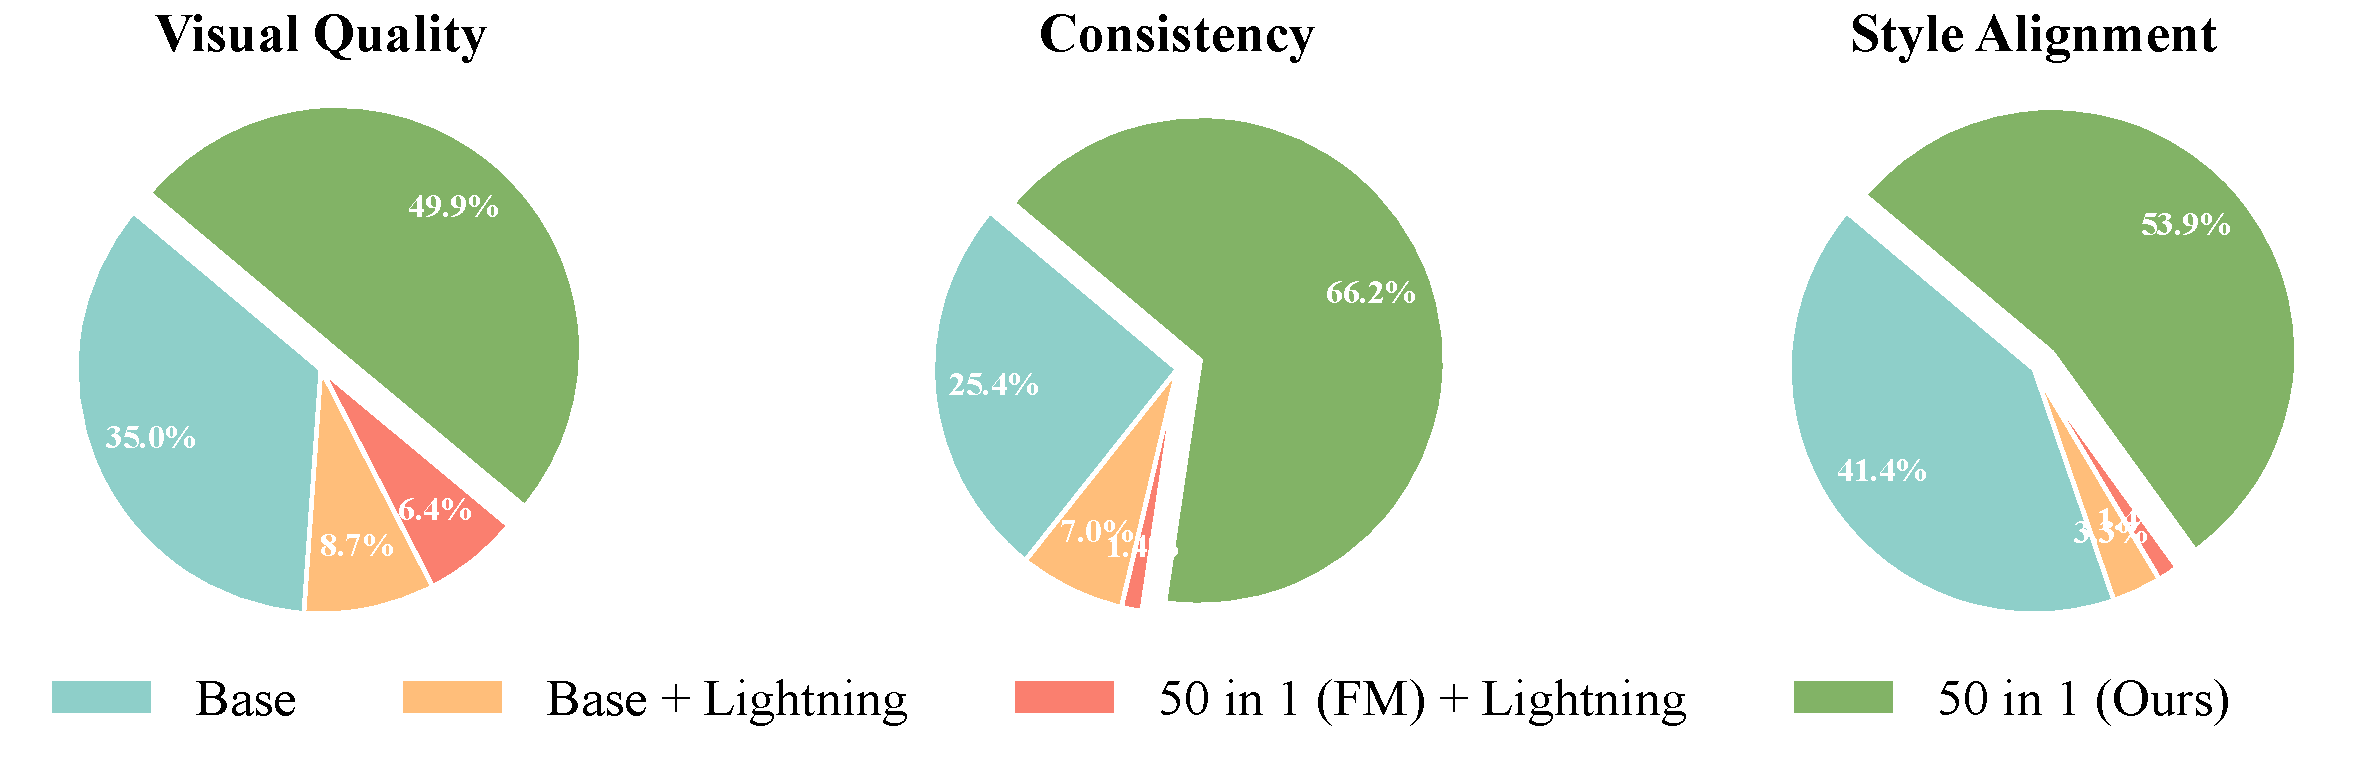
\includegraphics[width=\linewidth]{figures/user_study.pdf}
    \caption{\textbf{Detailed user study results.} Evaluators were asked to choose the best result among four candidates across three dimensions: Visual Quality, Consistency, and Style Alignment. Our proposed method, \textit{50 in 1 (Ours)}, consistently achieves the highest preference in all categories. Most notably, it secures 66.2\% of the votes for Consistency and 53.9\% for Style Alignment, significantly outperforming the \textit{Base} model and the \textit{Lightning} accelerated variants.}
    \label{fig:user_study_supp}
\end{figure}

\section{User Study and Additional Qualitative Results}
% 我们雇佣了10个专业的评估人员进行user study。具体来说，我们随机选取了50个测试样本对，每一对由原始图像、Base、Base+Lightning、50 in 1（FM）+ Lightning、Ours五个图像组成。评估人员在不知到测试样本真实标签的情况下接受测试，他们被要求从图像质量、一致性、风格对齐程度三个维度进行评估。即从4个候选图像中依次选出图像质量最好，一致性最好，风格对齐程度最好的那一个。评估结果如图X所示。
To subjectively evaluate our method, we conducted a user study involving 10 professional evaluators. We randomly sampled 50 test sets, where each set comprises the original reference image and four generated candidates: \textit{Base}, \textit{Base+Lightning}, \textit{50 in 1 (FM) + Lightning}, and \textit{Ours}. Evaluators were kept blind to the underlying methods. They were instructed to choose the best image among the four candidates based on three criteria: image quality, consistency, and style alignment. 
As shown in Figure~\ref{fig:user_study_supp}, we present the detailed preference distribution from our user study. Overall, our proposed method, \textit{50 in 1 (Ours)}, consistently outperforms all baseline methods across the three evaluated dimensions according to human perception.
Specifically, for \textbf{Visual Quality}, our method received the highest preference at 49.9\%, demonstrating that evaluators found our generated results to have superior visual appeal. The \textit{Base} model followed as the second most preferred with 35.0\% of the votes. 
In terms of \textbf{Consistency}, the advantage of our method is remarkably pronounced. It was selected as the best by a large margin of 66.2\%, indicating that our approach is highly effective in maintaining consistency compared to the alternatives. 
Regarding \textbf{Style Alignment}, our method again secured the majority of user preference (53.9\%), followed by the \textit{Base} model (41.4\%). Noticeably, the \textit{Lightning} variants (\textit{Base + Lightning} and \textit{50 in 1 (FM) + Lightning}) received minimal votes across all metrics. This suggests that while these variants might offer specific technical advantages, such as inference speed, they generally compromise subjective visual quality and stylistic fidelity. Ultimately, these results strongly validate that our method achieves the best overall balance of visual quality, consistency, and style alignment.

We provide additional visualization results in Figure~\ref{fig:visual1},~\ref{fig:visual2},~\ref{fig:visual3},~\ref{fig:visual4},~\ref{fig:visual5} and \ref{fig:visual6}.
\begin{figure*}[htb]
    \centering
    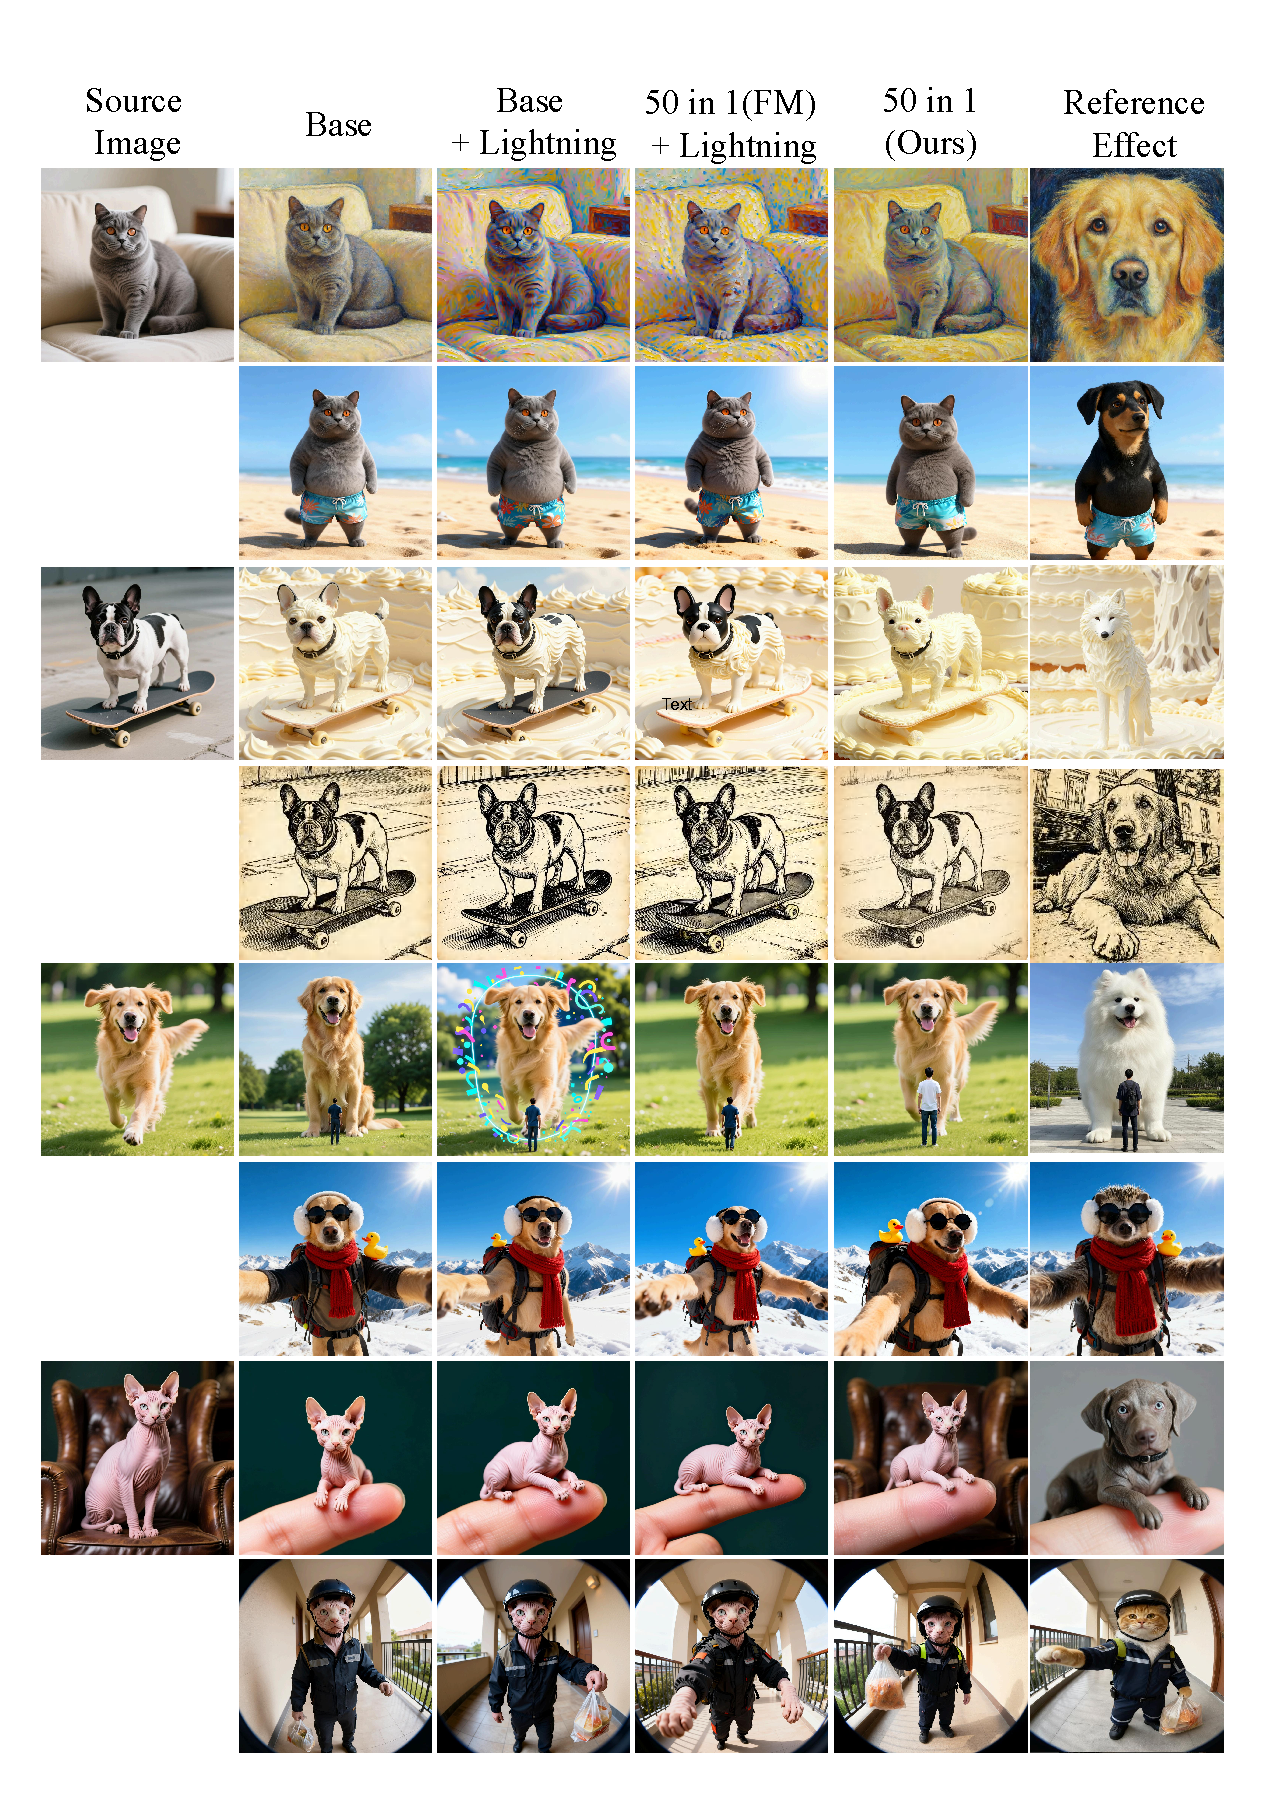
\includegraphics[width=\linewidth]{figures/visual2/zip_supp_v1.pdf}
    \caption{Qualitative Evaluation.}
    \label{fig:visual1}
    % \vspace{-0.5cm}
\end{figure*}

\begin{figure*}[htb]
    \centering
    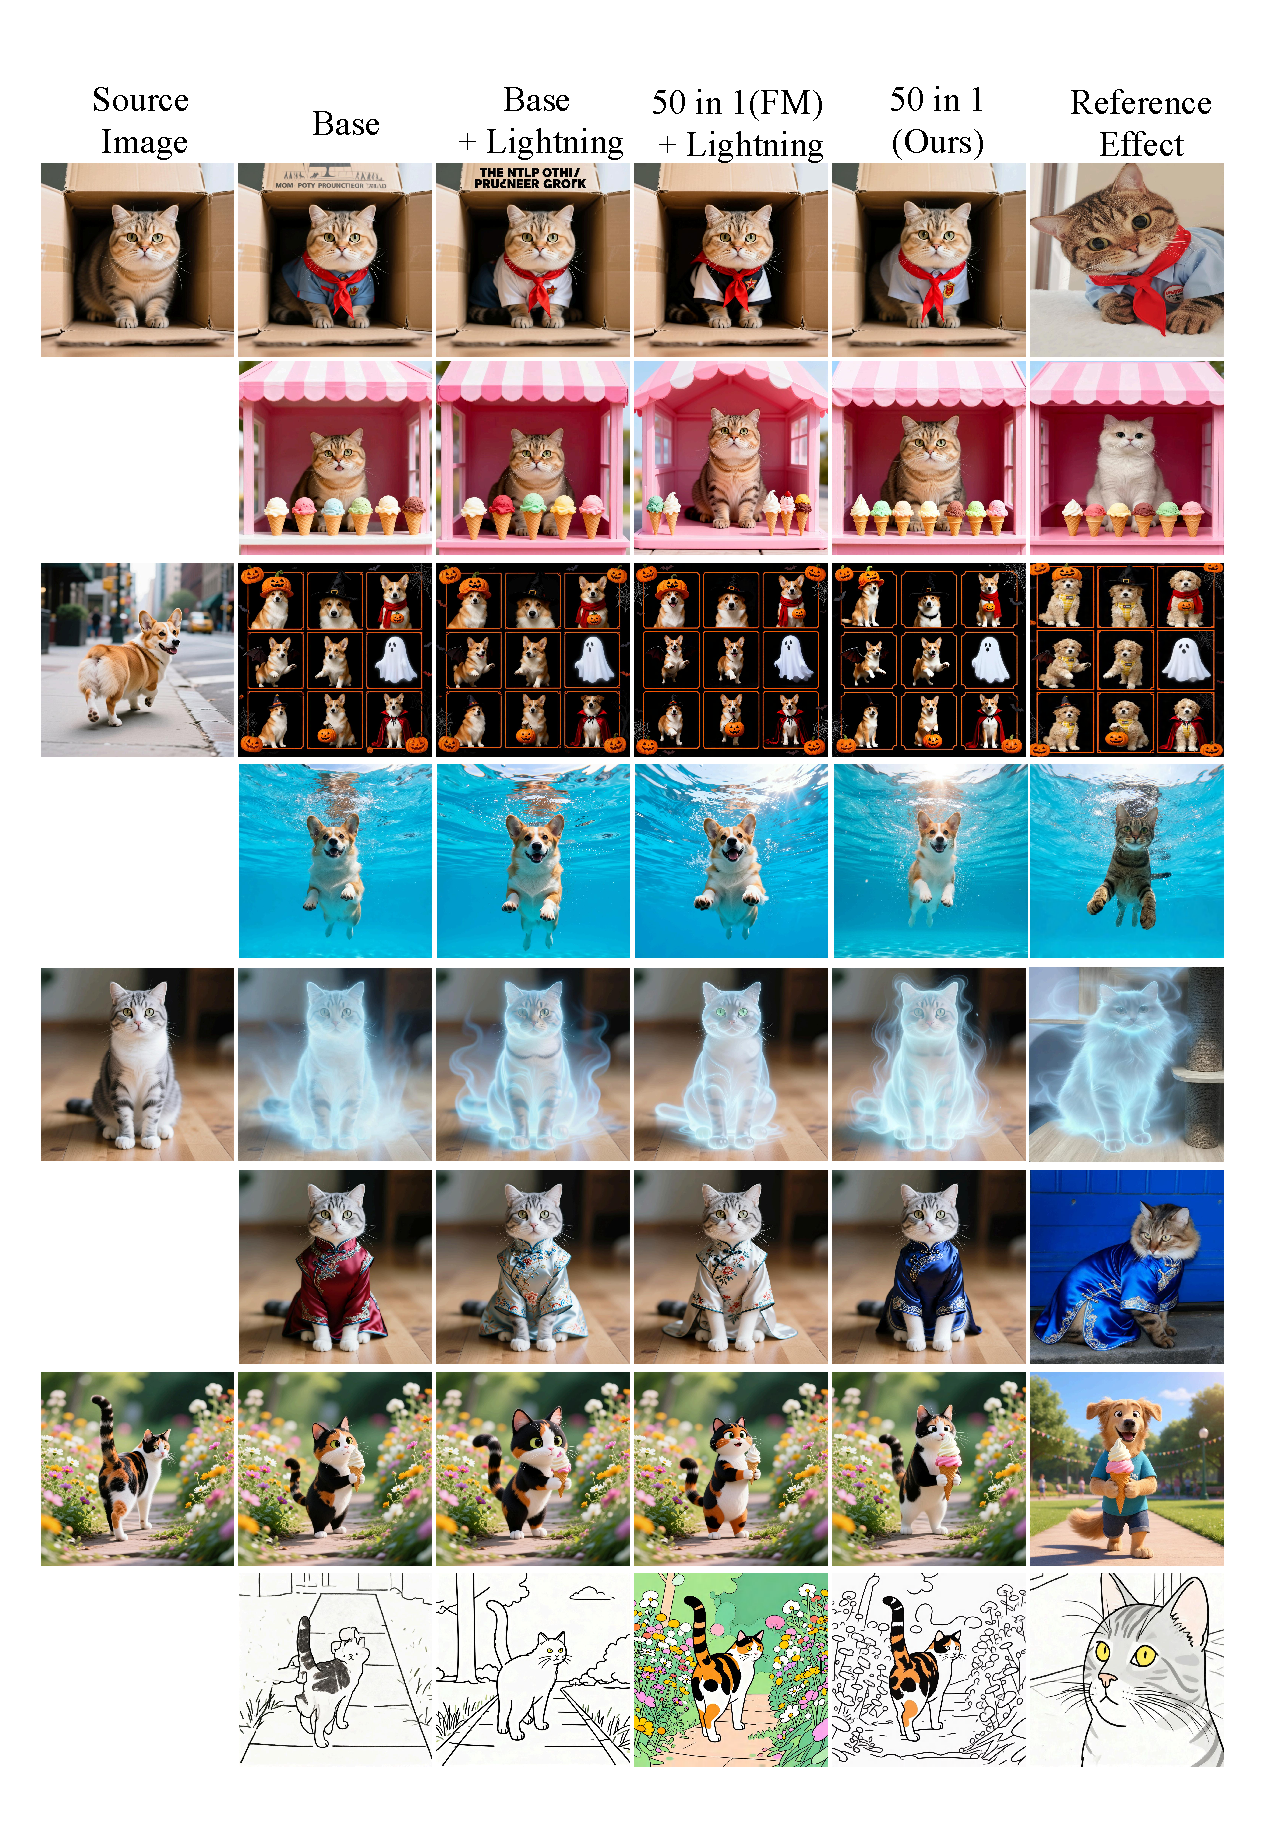
\includegraphics[width=\linewidth]{figures/visual2/zip_supp_v2.pdf}
    \caption{Qualitative Evaluation.}
    \label{fig:visual2}
    \vspace{-0.5cm}
\end{figure*}

\begin{figure*}[htb]
    \centering
    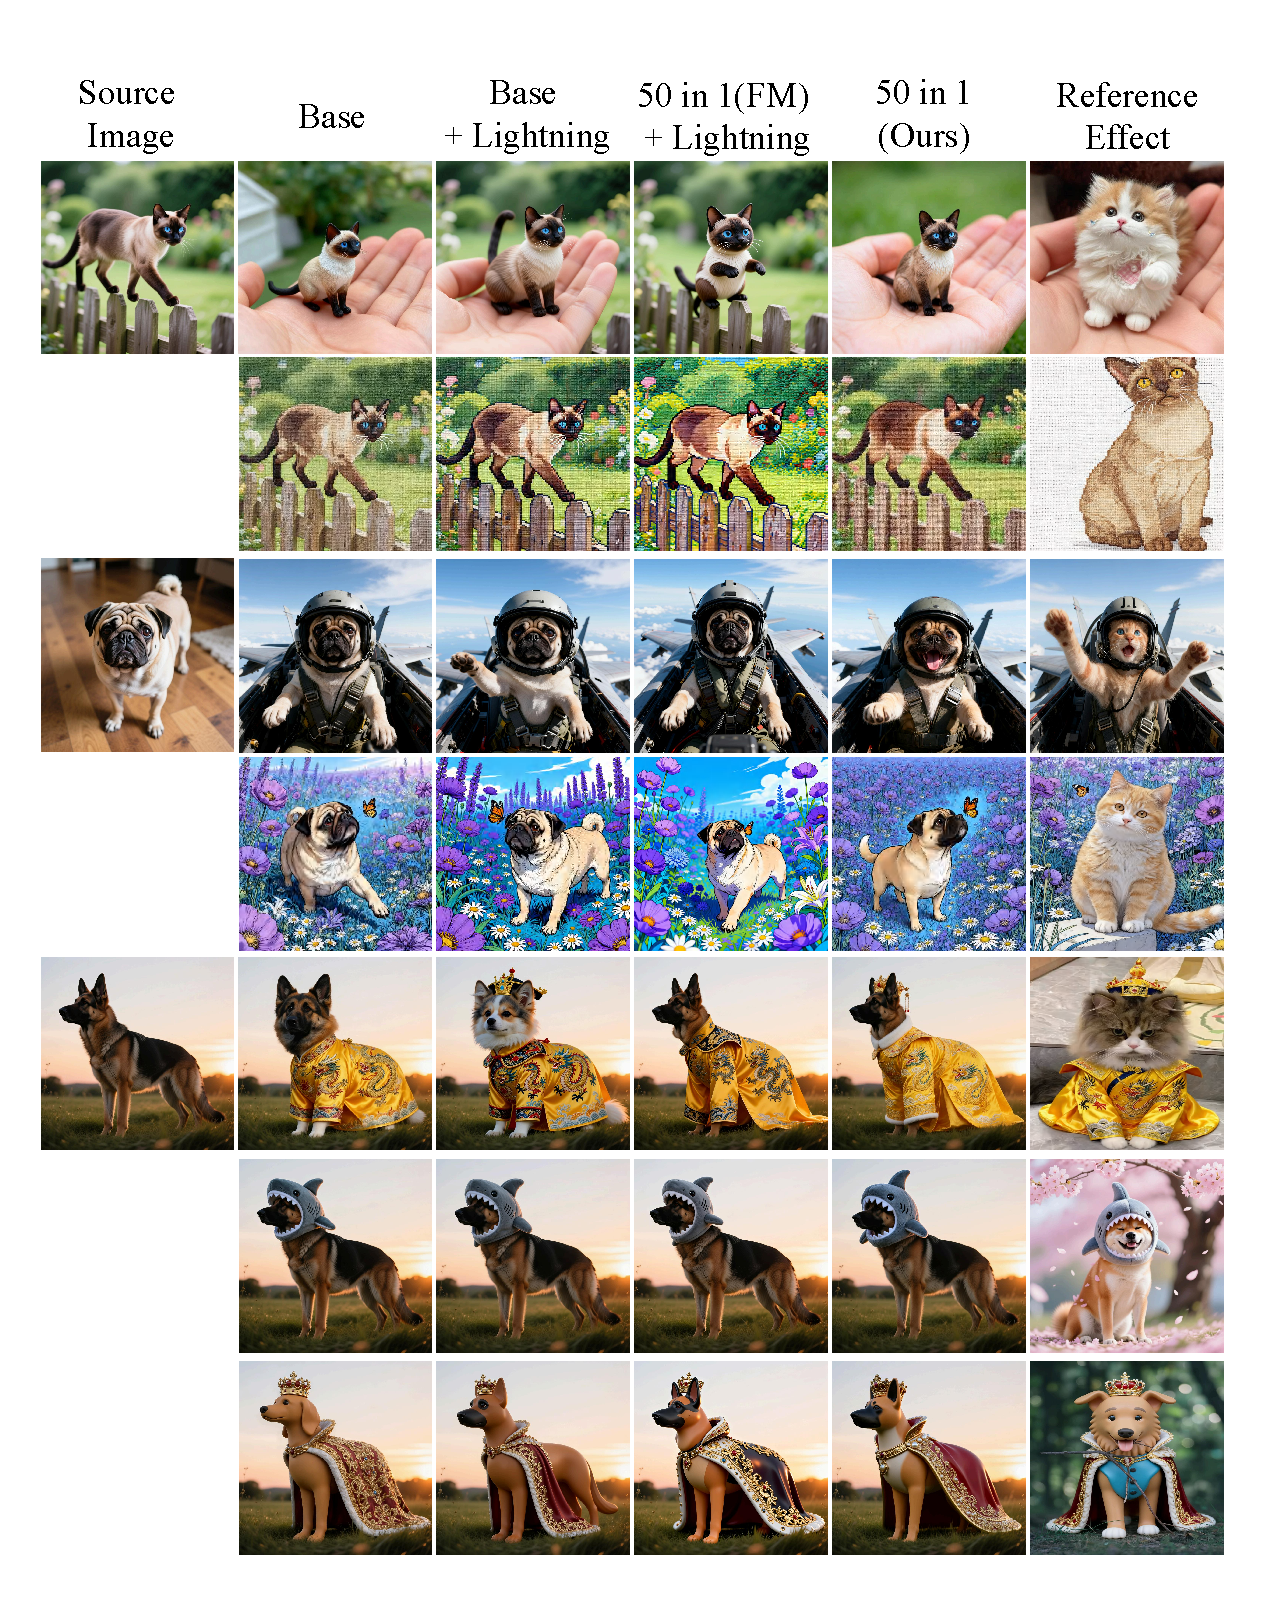
\includegraphics[width=\linewidth]{figures/visual2/zip_supp_v3_1.pdf}
    \caption{Qualitative Evaluation.}
    \label{fig:visual3}
    \vspace{-0.5cm}
\end{figure*}

\begin{figure*}[htb]
    \centering
    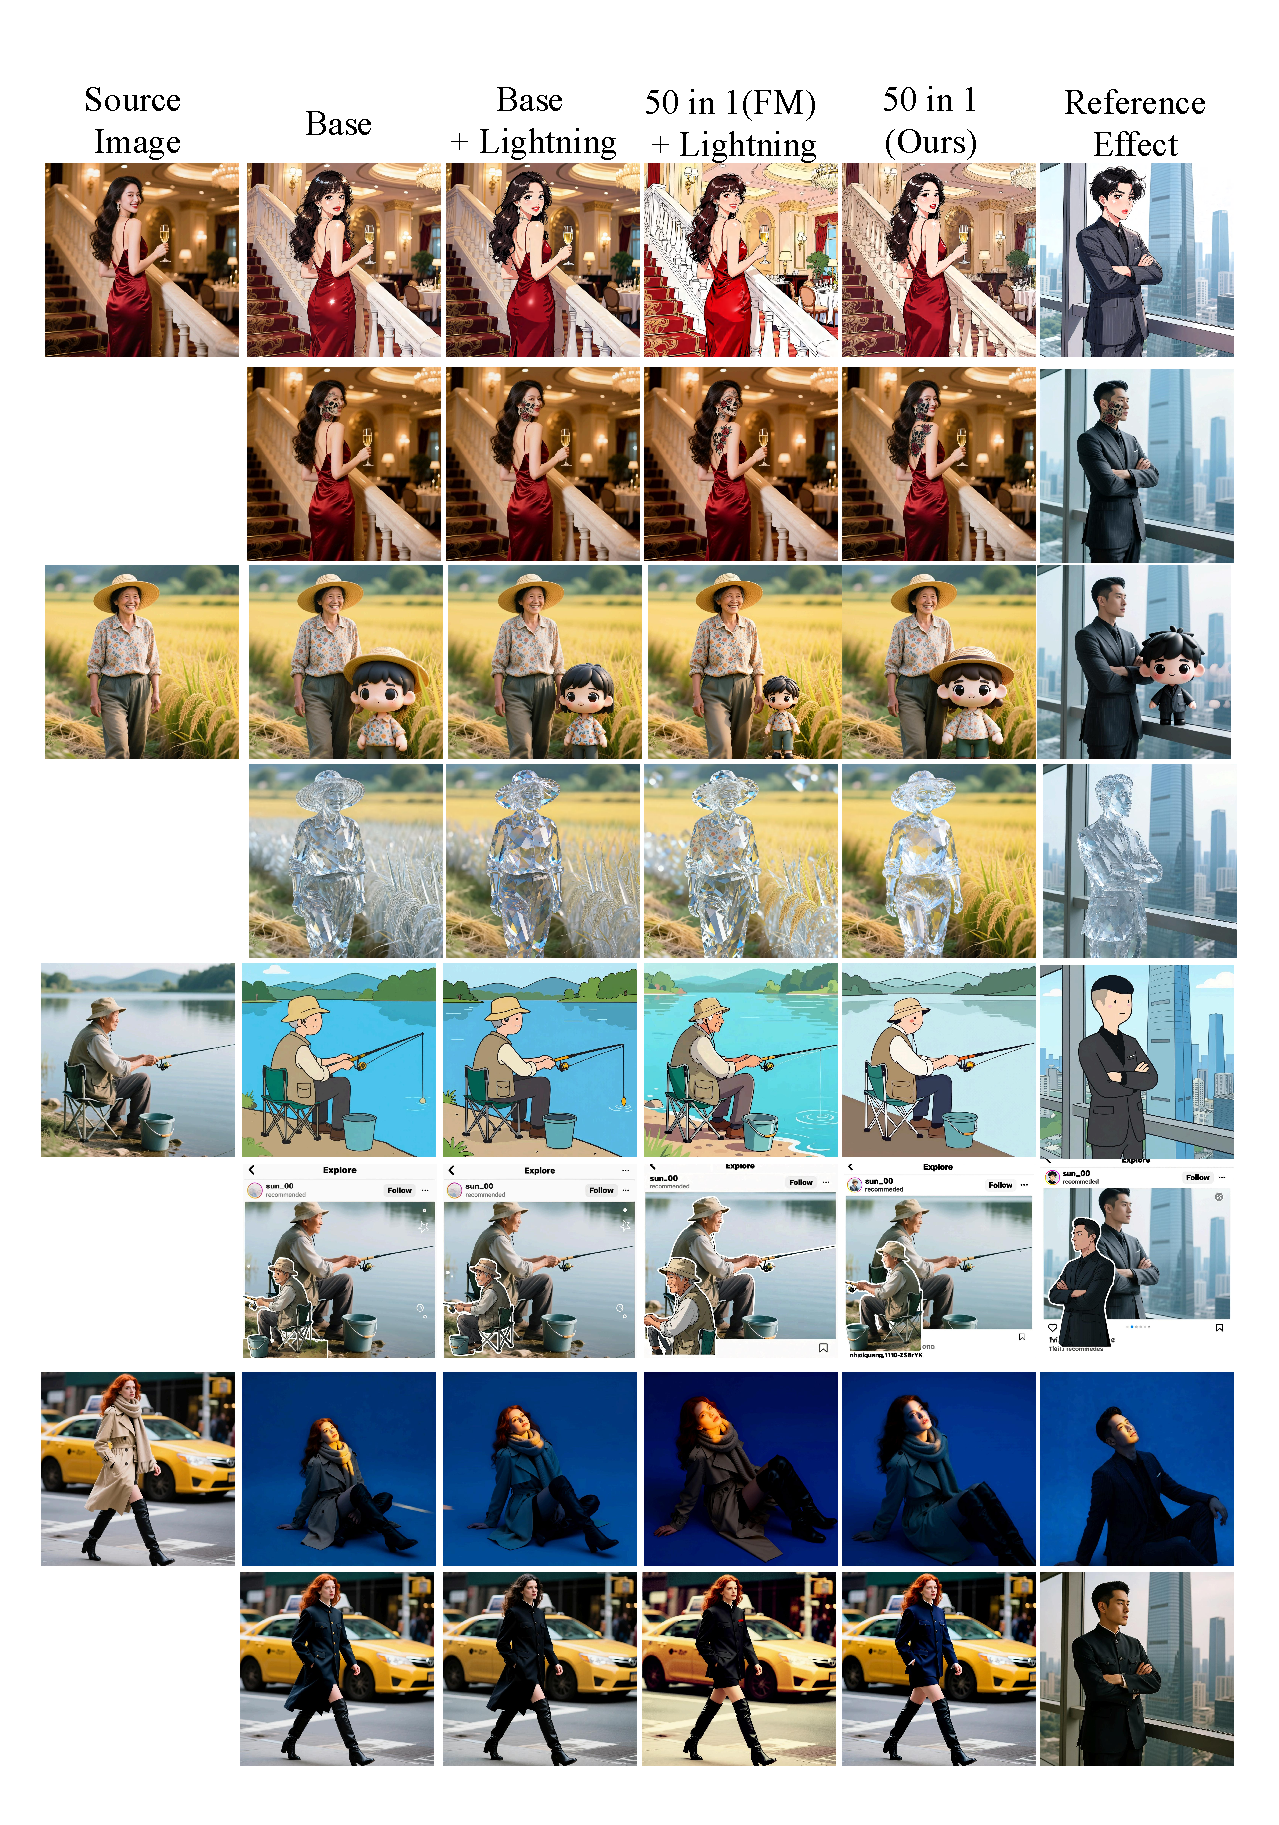
\includegraphics[width=\linewidth]{figures/visual2/zip_supp_v4.pdf}
    \caption{Qualitative Evaluation.}
    \label{fig:visual4}
    \vspace{-0.5cm}
\end{figure*}

\begin{figure*}[htb]
    \centering
    \includegraphics[width=\linewidth]{figures/visual2/zip_supp_v5.pdf}
    \caption{Qualitative Evaluation.}
    \label{fig:visual5}
    \vspace{-0.5cm}
\end{figure*}

\begin{figure*}[htb]
    \centering
    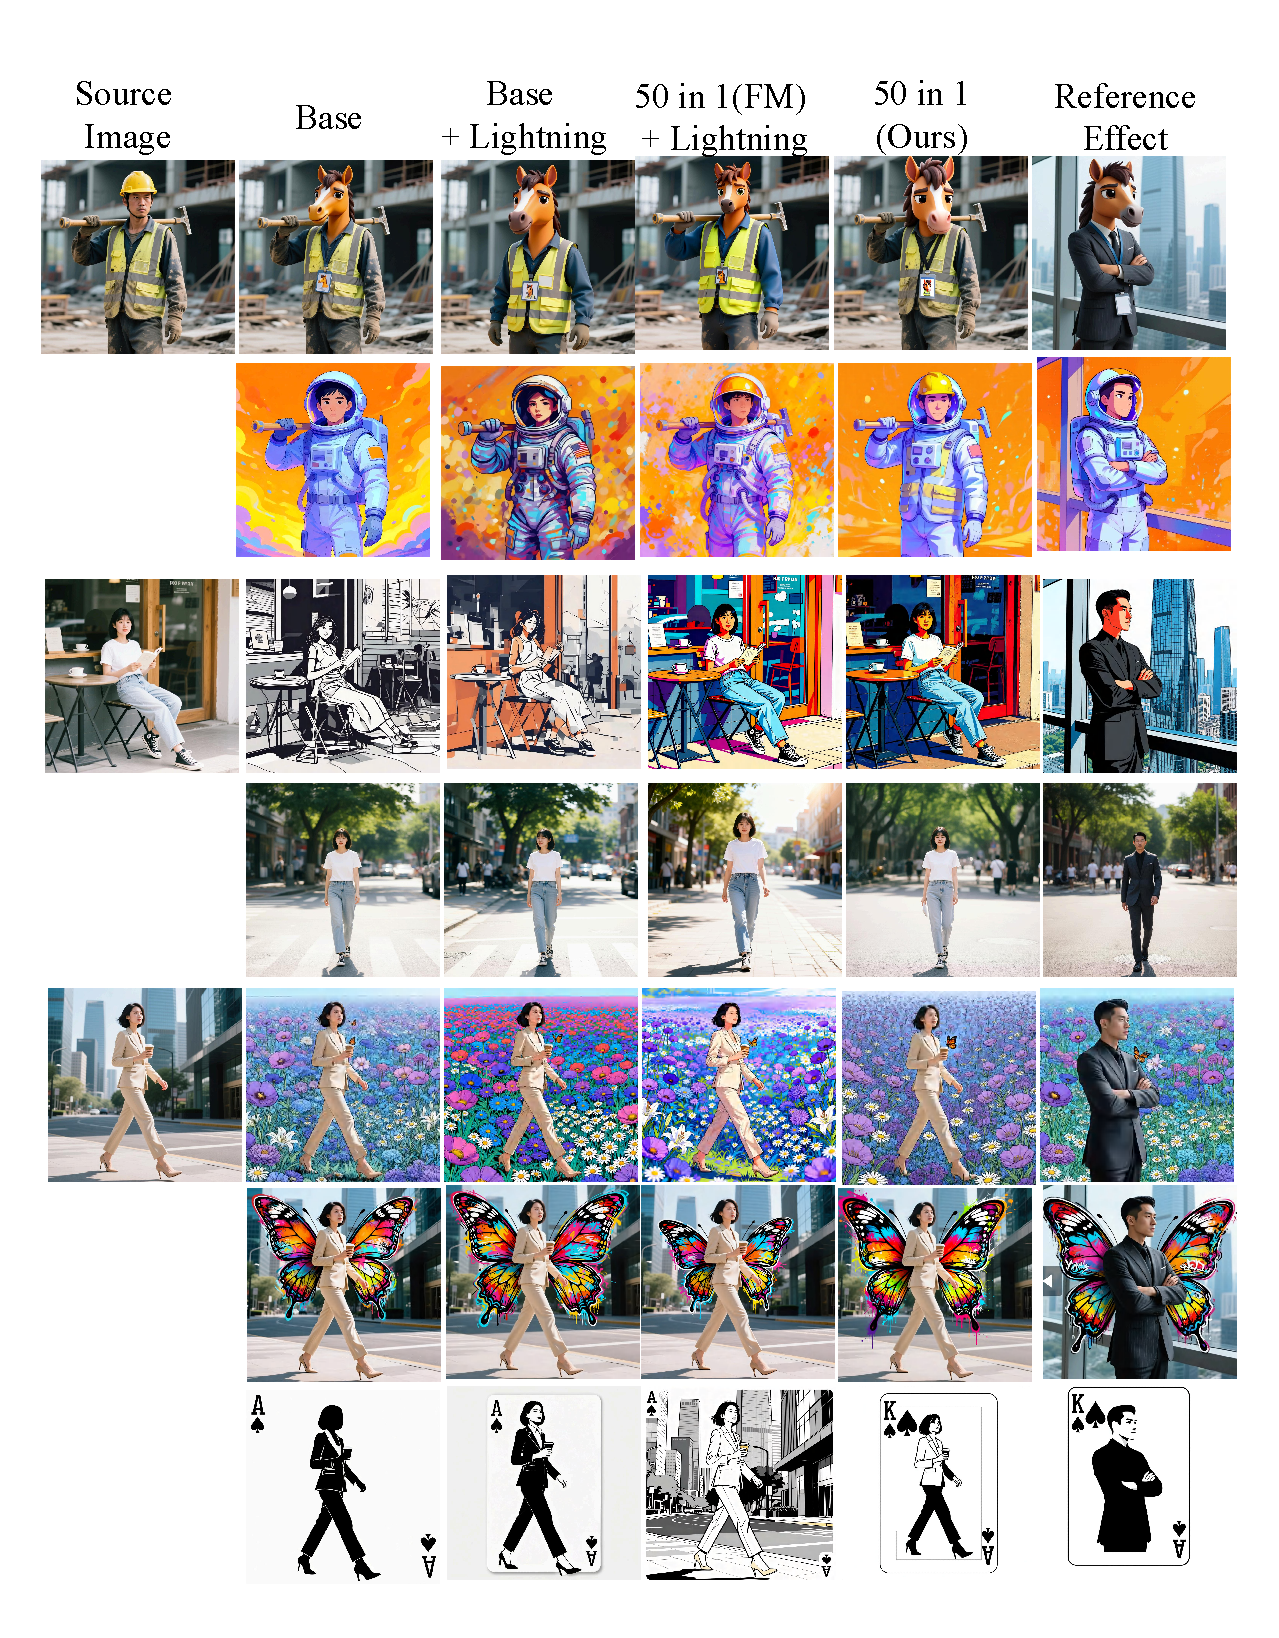
\includegraphics[width=\linewidth]{figures/visual2/zip_supp_v3_2.pdf}
    \caption{Qualitative Evaluation.}
    \label{fig:visual6}
    \vspace{-0.5cm}
\end{figure*}